% !TeX TS-program = xelatex
% This is SJTUBeamermin v1.0
% For more detailed desciption, see
% https://github.com/LogCreative/SJTUBeamermin/blob/main/doc/sjtubeamermintheme.pdf
%
\documentclass[
    % draft,                             % 草稿模式
    aspectratio=169,                   % 使用 16:9 比例
]{beamer}
\mode<presentation>
\usetheme[
    navigation=subsections,            % 使用子章节进度显示
     lang=en,                           % 使用英文
    % cjk=true,                          % 使用CJK而不是ctex
    color=blue,                         % 使用红色主题
    % pattern=all,                        % 使用全图案装饰
    % gbt=bibtex,                        % 使用 gbt (使用 bibtex 编译)
]{sjtubeamermin}
% \usecolortheme[]{beaver}                 % 使用其他颜色主题
% \addbibresource{ref.bib}               % gbt!=bibtex

\usepackage{amsmath,amsthm}
\usepackage{bm}
\usepackage{tikz-cd}
\usepackage{tikz}
\usetikzlibrary{trees,circuits.logic.US,circuits.ee.IEC}
\usepackage{empheq}
\usepackage{tabularx}
\usepackage{pifont}
\usepackage{multicol}
\usepackage[linesnumbered,ruled]{algorithm2e}
\usepackage{hyperref}
\usepackage{amsfonts}
\usepackage{tasks}
\usepackage{fontspec}
\usepackage{mdframed} % Add easy frames to paragraphs
\usepackage{color,soul}
\usepackage{xparse} % Add support for \NewDocumentEnvironment
\usepackage{biblatex}
\addbibresource{refs.bib}


\usepackage[customcolors]{hf-tikz}
\tikzset{style green/.style={
    set fill color=green!50!lime!60,
    set border color=white,
  },
  style cyan/.style={
    set fill color=cyan!90!blue!60,
  },
  style orange/.style={
    set fill color=orange!80!red!60,
  },
  hor/.style={
    above left offset={-0.31,0.31},
    below right offset={0.31,-0.2},
    #1
  },
  ver/.style={
    above left offset={-0.1,0.3},
    below right offset={0.15,-0.15},
    #1
  }
}

\renewcommand{\Bbb}{\mathbb}
\newcommand{\Z}{\mathbb{Z}}
\newcommand{\GR}{\mathbb{GR}}
\newcommand{\F}{\mathbb{F}}
\newcommand{\R}{\mathbb{R}}
\newcommand{\Fns}{\mathbb{F}_{2^n}^*}
\newcommand{\Fn}{\mathbb{F}_{2^n}}
\newcommand{\Fks}{\mathbb{F}_{2^k}^*}
\newcommand{\Fk}{\mathbb{F}_{2^k}}
\newcommand{\df}{\delta_F}
\newcommand{\tr}{\operatorname{tr}_1^k}
\newcommand{\gtr}{\operatorname{T}}
\newcommand{\Bn}{\mathcal{B}_n}
% The symbol of sharing
\newcommand{\Sh}{\operatorname{Sh}}
% The symbol of Teichmuller sets
\newcommand{\teich}{\textit{Teichm$\ddot{u}$ller sets}}

% \newtheorem*{definition}{Definition}
\newtheorem{thm}{Theorem}
\newtheorem{lem}[thm]{Lemma}
\newtheorem{proposition}{Proposition}
\definecolor{graylight}{cmyk}{.30,0,0,.67} % define color using xcolor syntax
\setbeamertemplate{itemize items}[default]

% modify the footnote symbol 
% \makeatother
% \renewcommand{\thefootnote}{\ifcase\value{footnote}\or\dagger\or(\#\#)\or(\#\#\#)\or(\#\#\#\#)\or(\#\#\#\#\#)\fi}
% \makeatletter



\newmdenv[ % Define mdframe settings and store as leftrule
  linecolor=red,
  topline=false,
  bottomline=false,
  rightline=false,
  skipabove=\topsep,
  skipbelow=\topsep
]{leftrule}

% \NewDocumentEnvironment{example}{O{\textbf{Example:}}} % Define example environment
% {\begin{leftrule}\noindent\textcolor{blue}{#1}\par}
% {\end{leftrule}}
\setbeamertemplate{footline}[frame number]

\NewDocumentEnvironment{question}{O{\textbf{Something:}}} % Define something environment
{\begin{leftrule}\noindent\textcolor{graylight}{#1}\par}
{\end{leftrule}}

\NewDocumentEnvironment{remark}{O{\textbf{Remark:}}} % Define remark environment
{\begin{leftrule}\noindent\textcolor{blue}{#1}\par}
{\end{leftrule}}

\begin{document}
    \institute[School of Electronic Information and Electrical Engineering]{电子信息与电气工程学院}   % 组织
    % \logo{
    %     \includegraphics{support/cnlogored.pdf}  % 重定义 logo
    % }
    \titlegraphic{                         % 标题图像
        \begin{stampbox}[white]
            \includegraphics[width=0.3\textwidth]{support/head.png}
        \end{stampbox}
    }
    \title{Threshold Implementations\\ of Bijective Sboxes}  % 标题
 %   \subtitle{SJTUBeamer \fbox{\textsc{min}} Template}         % 副标题
    \author{Zhaole Li}                  % 作者
    \date{\textcolor{red}{2023/3/8}}                          % 日期
    \maketitle                             % 创建标题页


\AtBeginSection[]{
   \begin{frame}
       % \tableofcontents[currentsection]           % 传统节目录             
       \sectionpage                   % 节页
   \end{frame}
}

% 使用小节目录
%\AtBeginSubsection[]{                  % 在每小节开始
 %   \begin{frame}
        % \tableofcontents[currentsection,currentsubsection]             % 传统小节目录             
  %      \subsectionpage                % 小节页
 %   \end{frame}
%}

\section{Introduction}
%\subsection{第 1 小节}
    \begin{frame}
        \frametitle{Differential Power Analysis in SCA}
        \begin{itemize}
            \item Side-channel attacks (SCA) exploit information that leaks from cryptographic devices 
            and power analysis is one form of those attacks.
            \item Power analysis uses a physical device's power consumption that maybe leak some information to derive secret keys.
            \item Differential power analysis (DPA) and simple power analysis are two main approaches.
            \item `Differential' means finding the difference between two results of the intermediates in a cryptographic calculation, 
            for example, for the least-significant bit (LSB) of the Sbox in AES in round $ 1 $, the difference 
            of results when LSB was $ 1 $ and LSB was $ 0 $. 
        \end{itemize}

    \end{frame}

    \begin{frame}
        \frametitle{Masking}
        \begin{itemize}
            \item To against DPA attacks, a commonly used approach is to make the intermediate results of algorithms executing independent with the secret keys by randomizing all intermediate results.
            \item One of the most widely used techniques to secure an implementation is secret sharing, 
            as known as masking.
            \item However, glitches that occur in circuits also lead to a side-channel leakage and a glitch-free hardware is expensive.  
            \item Note that the linear transformation is easy to mask, we only focus on nonlinear transformations. 
        \end{itemize}
    \end{frame}

    \begin{frame}
        \frametitle{Glitches Can Leak Information}

        \begin{example}
            
            Consider AND gate with $ x,y $ are inputs and $ z $ is output. 
            Assume a glitch occurs in $ x $. If input $ y $ is $ 1 $, then $ z=x\land y=x $, and the glitch in $ x $ will 
            change the state temporarily. But when $ y=0 $, the glitch in $ x $ will not affect the output. Consequently, 
            the glitch in $ x $ depends on the value of $ y $.
            \begin{table}
                \caption{Glitches in $ x $ leak information in $ z=x\land y $}
                $\begin{array}{|ll|c|}
                    \hline 
                    y & \widetilde{x} & \widetilde{z} \\
                    \hline 
                    0 & 0 & 0  \\
                    0 & 1 & 0  \\
                    1 & 0 & 0  \\
                    1 & 1 & 1  \\
                    \hline
                \end{array}$
            \end{table}

            Denote $ \widetilde{x} $ a glitch in $ x $. $ \widetilde{x}=0 $ means no glitch occurs in $ x $ and otherwise if 
            $ \widetilde{x}=1 $.
        \end{example}
    \end{frame}

    \begin{frame}
        \frametitle{A Masked AND-Gate}
            Consider an implementation of a masked AND-Gate. 
            The circuit takes $ 5 $ inputs: two random masks $ a,b $, two masked inputs $ \widetilde{x} = a\oplus x, \widetilde{y} = b\oplus y$, and a new random value $ c $ to mask the output $ z = x \land y $. 
            Therefore the circuit's output is computed as follows: 
            \[\widetilde{z}=\widetilde{x} \widetilde{y} \oplus(b \widetilde{x} \oplus(a \widetilde{y} \oplus(a b \oplus c))).\]

        \begin{figure}
                \centering
            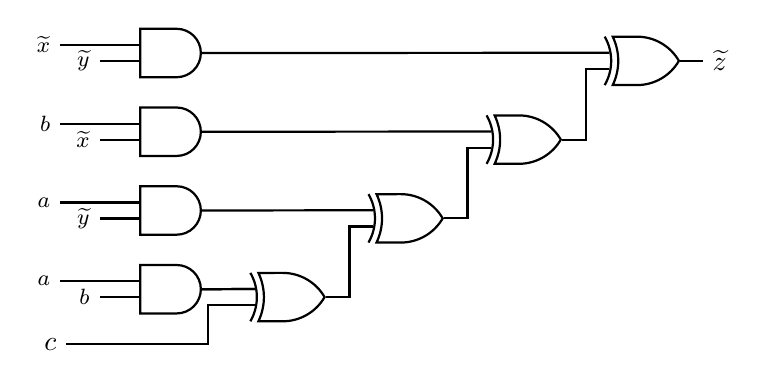
\begin{tikzpicture}[circuit logic US, every circuit symbol/.style={thick}]
                \node[and gate,inputs={nn}, point right] (and1) at (0,-1)  {};
                \node[and gate,inputs={nn}, point right] (and2) at (0,0)  {};
                \node[and gate,inputs={nn}, point right] (and3) at (0,1)  {};
                \node[and gate,inputs={nn}, point right] (and4) at (0,2)  {};
                \node[xor gate,inputs={nn}, point right] (xor4) at (6,1.9)  {};
                \node[xor gate,inputs={nn}, point right] (xor3) at (4.5,0.9)  {};
                \node[xor gate,inputs={nn}, point right] (xor2) at (3,-0.1)  {};
                \node[xor gate,inputs={nn}, point right] (xor1) at (1.5,-1.1)  {};
                \node (c_input) at (-1.5,-1.7) {$ c $};
                \node (z_output)  [right of = xor4] {$ \widetilde{z} $};
                
                \draw [black,thick] (and1.input 1) -- ++(left:1) node [left]{\footnotesize $ a $};
                \draw [black,thick] (and1.input 2) -- ++(left:.5) node [left]{\footnotesize $ b $};
                \draw [black,thick] (and2.input 1) -- ++(left:1) node [left]{\footnotesize $ a $};
                \draw [black,thick] (and2.input 2) -- ++(left:.5) node [left]{\footnotesize $ \widetilde{y} $};
                \draw [black,thick] (and3.input 1) -- ++(left:1) node [left]{\footnotesize $ b $};
                \draw [black,thick] (and3.input 2) -- ++(left:.5) node [left]{\footnotesize $ \widetilde{x} $};
                \draw [black,thick] (and4.input 1) -- ++(left:1) node [left]{\footnotesize $ \widetilde{x} $};
                \draw [black,thick] (and4.input 2) -- ++(left:.5) node [left]{\footnotesize $ \widetilde{y} $};
                
                \draw [black,thick] (and4.output) --  (xor4.input 1);
                \draw [black,thick] (and3.output) --  (xor3.input 1);
                \draw [black,thick] (and2.output) --  (xor2.input 1);
                \draw [black,thick] (and1.output) --  (xor1.input 1);
                \draw [black,thick] (and1.output) --  (xor1.input 1);
                \draw [black,thick] (xor1.output) -- ++(right:3mm) |- (xor2.input 2);
                \draw [black,thick] (xor2.output) -- ++(right:3mm) |- (xor3.input 2);
                \draw [black,thick] (xor3.output) -- ++(right:3mm) |- (xor4.input 2);
                \draw [black,thick] (c_input) -- ++(right:2cm) |- (xor1.input 2);
                \draw [black,thick] (xor4.output) -- (z_output);
            \end{tikzpicture}
            \caption{A masked AND-Gate}
        \end{figure}
    \end{frame}
        
    \begin{frame}
        \frametitle{Glitches in a Masked AND-Gate}
        Consider what happens if a glitch occurs in input $ \widetilde{x} $. 
        The influence of this glitch depends on the values of $ b $ and $ \widetilde{y} $, 
        then, we have a table of the number of affected gates in the masked AND-Gate: 
        \begin{table}
            \caption{Number of affected gates in the circuit of the masked AND-Gate, when a glitch occurs in input $ \widetilde{x} $}
            $\begin{array}{|cc|cc|}
                \hline 
                b & \widetilde{y} & \text { AND } & \text{ XOR } \\
                \hline
                0 & 0 & 0 & 0 \\
                0 & 1 & 1 & 1 \\
                1 & 0 & 1 & 2 \\
                1 & 1 & 2 & 2 \\
                \hline
            \end{array}$
        \end{table}
    \end{frame}

    \begin{frame}
        \frametitle{Glitches in a Masked AND-Gate also Leak Information}
        \begin{itemize}
            \item The energy consumption caused by the glitch is related to the number of gates that exist the glitch. 
            \item It's clear from the table above that energy consumption depends on the values of $ b $ and $ \widetilde{y} $. 
            \item Since in general the mean energy consumption is different for $ y=0 $ and $ y=1 $, 
            the energy consumption will leaks information on the value of $ y $. 
            \item Similar results can be obtained by analyzing the effect of a glitch in one of the other inputs. 
        \end{itemize}
            
    \end{frame}

    \begin{frame}
        \frametitle{Threshold Implementations (TI)}
        \begin{itemize}
            \item Threshold Implementations, a method to against DPA attacks and glitches, based on ideas of multiparty computation. 
            \item In the TI of an $ (n,m) $-function $ F $,  the shares of the output of $ F $ are the outputs of several functions of the shares of the input (correctness), each function being independent of at least one of the shares of the input to $ F $ (non-completeness). 
            \item The property, called uniformity, is also essential to be against DPA, since it holds that the mean 
            energy consumption is constant. 
            \item We say that $ \mathcal{F} $ is a $ d $-th order threshold implementation of $ F: \F_2^n\rightarrow \F_2^m $ if $ \mathcal{F} $ is correct with respect to $ F $, $ d $-th order non-complete, and uniform.
        \end{itemize}
    \end{frame}

    \begin{frame}
        \frametitle{Sharing}
        
        \begin{definition}
            An $ s $-sharing of $ x\in\F $ is a tuple $ \underline{x}=(x_1,...,x_s)\in\F^s $ over $ \F $ such that 
            \[x=\sum_{i=1}^{s}x_i.\]
            The value $ x $ can be interpreted as the secret, and $ x_1,...,x_s $ as the shares.
        \end{definition}
        
        For every $ x\in\F $, we define the set of $ s $-sharings of $ x $ as 
        \[\operatorname{Sh}_s(x)=\left\{ \underline{x}=(x_1,...,x_s)\in\F^s\middle|\sum_{i=1}^{s}x_i=x \right\}.\]
        
    \end{frame}

    \begin{frame}
        \frametitle{Correctness and Non-completeness in TI}
        \begin{definition}[Correctness]
            Let $ s_x,s_y $ be positive integers and $ \mathcal{F}:(\F_2^n)^{s_x}\rightarrow(\F_2^m)^{s_y} $ be an $ s_x $ to $ s_y $ sharing, where $ \mathcal{F}(\underline{x})=\left( F_1(\underline{x}),F_2(\underline{x}),...,F_{s_y}(\underline{x}) \right) $ 
            and $ F_i $ are $ (s_x\times n,m) $-functions.
            We say that $ \mathcal{F} $ is correct, or equivalently that it has the correctness property, 
            with respect to $ F:\F_{2^n}\rightarrow\F_{2^m} $, if for all $ x\in\F_{2^n} $ and $ \underline{x}\in\operatorname{Sh}_{s_x}(x) $, 
            we have 
            \[\mathcal{F}(\underline{x})\in\operatorname{Sh}_{s_y}(F(x)).\]
        \end{definition}
        \begin{definition}[$ d $-th Non-completeness]
            We say that $ \mathcal{F} $ is $ d $-th order non-complete, if every coordinate function $ \mathcal{F}_i $ is independent of at least $ d $ share of all input variables $ x_1,...,x_{s_x} $. 
        \end{definition}
        For $ d=1 $, we use non-complete instead of the first order non-complete. 
    
    \end{frame}
    \begin{frame}
        \frametitle{Correctness and Non-completeness in TI}
        
        \begin{example}[Correctness and non-completeness]
            Consider the multiplication of two operands in the finite field $ \F_2 $: $ z=xy $. 
            Let the number of shares $ n = 3 $, i.e. $ x=(x_1,x_2,x_3),y=(y_1,y_2,y_3) $ and $ z=(z_1,z_2,z_3) $. 
            Define the three coordinate functions $ f_i $ as follows:
            \begin{align*}
                 z_1&=F_1\left(x_2, x_3, y_2, y_3\right)=x_2 y_2 \oplus x_2 y_3 \oplus x_3 y_2 \\
                 z_2&=F_2\left(x_1, x_3, y_1, y_3\right)=x_3 y_3 \oplus x_1 y_3 \oplus x_3 y_1 \\
                 z_3&=F_3\left(x_1, x_2, y_1, y_2\right)=x_1 y_1 \oplus x_1 y_2 \oplus x_2 y_1.
            \end{align*}
            Clearly the computation of the output share $ z_i $ is independent of $ x_i,y_i $, 
            then $ z_i $ cannot correlate with inputs $ x,y $, thus we ensure that no correlation to the output exists. 
            And correctness is easy to verify. 
        \end{example}
    \end{frame}
    
    \begin{frame}
        \frametitle{Uniformity in TI}
        \begin{itemize}
            \item A realization $ \mathcal{F} $ is uniform if for all values of $ x\in\F_2^n $ and $ \underline{y}\in\operatorname{Sh}_{s_y}(F(x)) $ the following holds:
            \[\lvert\left\{ \underline{x}\in\operatorname{Sh}_{s_x}(x)\middle|\mathcal{F}(\underline{x})=\underline{y} \right\}\rvert=\frac{2^{n(s_x-1)}}{2^{m(s_y-1)}}.\]
            \item When $ s_x=s_y $ and $ F $ is a permutation, $ \mathcal{F} $ being uniform is equivalent to $ \mathcal{F} $ being a permutation. 
            \item Uniformity is the hard property among the three described above, for example, there is no TI  realization for multiplication satisfying uniform with $ 3 $ shares only. 
            \item If we use a nonuniform TI of a function, we need to add sufficient fresh randomness or to change the guards.  
        \end{itemize}
    \end{frame}

    \begin{frame}
        \frametitle{A TI of Multiplication in $ \F_2 $}
        \begin{example}
            The following TI realization with $ 4 $ shares satisfies three properties with $ x=(x_1,x_2,x_3,x_4)\in(\F_2)^4,y=(y_1,y_2,y_3,y_4)\in(\F_2)^4 $ and $ z=(z_1,z_2,z_3,z_4)\in(\F_2)^4 $: 
            \begin{align*}
                z_1&=\left(x_3 \oplus x_4\right)\left(y_2 \oplus y_3\right) \oplus y_2 \oplus y_3 \oplus y_4 \oplus x_2 \oplus x_3 \oplus x_4 \\
                z_2&=\left(x_1 \oplus x_3\right)\left(y_1 \oplus y_4\right) \oplus y_1 \oplus y_3 \oplus y_4 \oplus x_1 \oplus x_3 \oplus x_4 \\
                z_3&=\left(x_2 \oplus x_4\right)\left(y_1 \oplus y_4\right) \oplus y_2 \oplus x_2 \\
                z_4&=\left(x_1 \oplus x_2\right)\left(y_2 \oplus y_3\right) \oplus y_1 \oplus x_1.
            \end{align*}
        \end{example}
        \begin{remark}
            With uniformity, we need one more share and more complicated formulas.
        \end{remark}
    \end{frame}

    

\section{A Universal Construction for the TI for Bijective Sboxes} 
    \begin{frame}
        \frametitle{A Universal Construction for the TI with $ t + 2 $ Shares}
    
        \begin{itemize}
            \item For a bijective Sbox of algebraic degree at most $ t $, Piccione et al. give a general $ (t+2) $-shares first order TI construction.  
            This construction does not depend on the dimension $ n $ of vector space $ \F_2^n $ where $ F $ permutes. 
            \item The authors focus on the first order TI of permutation with $ s_x=s_y $. 
            Although a lower bound on the number of shares to achieve a  first order TI for some $ F $ is $ s\ge\deg(F)+1 $, 
            the theoretically smallest number of shares $ t + 1 $ is not possible for all Sboxes, 
            so their construction is the first optimal universal TI construction for some bijective Sboxes. 
            \item By adding coordinate terms, the new function obtained still satisfies non-complete.
        \end{itemize}
    \end{frame}

    \begin{frame}
        \frametitle{TI of Inversion over Finite Fields}
        \begin{itemize}
            \item Inversion in $ \F_{2^4} $ has algebraic degree $ 3 $, then we need at least $ 3+1=4 $ shares to implement this function. 
            However, exhaustive search revealed that no realization with $ 4 $ shares can satisfy uniform. 
            \item The AES Sbox, inversion in $ \F_{2^8} $,  has algebraic degree $ 7 $. 
            The implementations on the AES Sbox as applications of the construction have low latency and no randomness. 
            \begin{table}
                \caption{Hardware cost of the masked AES S-box in the NANGATE $ 45 $ nm library}    
                $\begin{array}{lccc}
                \hline \text { Design } & \text { Area }[kGE] & \text { Latency }[cc] & \text { Randomness }[bits] \\
                \hline \text { This construction } & 128.27 & 1 & 0 \\
                \text { This construction} [(x^{26})^{49}] & 21.86 & 2 & 0 \\
                \text { Wegener-Moradi } & 4.20 & 16 & 0 \\
                \text { Sugawara } & 3.50 & 4 & 0 \\
                \text { Gross et al. } & 60.76 & 1 & 2048 \\
                \text { Gross et al. } & 6.74 & 2 & 416 \\
                \hline
            \end{array}$
        \end{table}

        \end{itemize}
    
    \end{frame}
    
    \begin{frame}
        \frametitle{A Universal Construction}
    
        Let $\mathcal{F}:\left(\mathbb{F}_2^n\right)^{t+2} \rightarrow\left(\mathbb{F}_2^n\right)^{t+2}$ be defined for every $\underline{x}=\left(x_1, \ldots, x_{t+2}\right) \in\left(\mathbb{F}_2^n\right)^{t+2}$ as
        \[
        \mathcal{F}(\underline{x})=\left(\begin{array}{rl}
        \mathcal{F}_1(\underline{x})= & x_1 \\
        \mathcal{F}_2(\underline{x})= & \sum_{i=3}^{t+2} x_i+F\left(\sum_{i=2}^{t+2} x_i\right) \\
        \mathcal{F}_j(\underline{x})= & x_j+\sum_{I \in \mathcal{I}_{j-2}} F\left(\sum_{i \in I} x_i+\sum_{i=j}^{t+2} x_i\right) \\
        & j=3, \ldots, t+1 \\
        \mathcal{F}_{t+2}(\underline{x})= & x_{t+2}+x_1+\sum_{I \in \mathcal{I}_t} F\left(\sum_{i \in I} x_i\right)
        \end{array}\right)^{\mathrm{T}},
        \]
        where for any $k \geq 1$ we denote by $\mathcal{I}_k$ as the set of all subsets of $\{1, \ldots, k\}$ (including $\emptyset$). Moreover, we use the convention that $\sum_{i \in \emptyset} x_i=0$.
    
    \end{frame}

    \begin{frame}
        \frametitle{Decompose $ F $ into several parts}
    
     The method they used is below, that is, to decompose the 
    $ F(\sum_{i=1}^{t+2}x_i) $ into the sum of several partial sums of the shares within $ t $:
    \begin{lemma}
      Let $ F:\F_2^n\rightarrow\F_2^m $ be of algebraic degree at most $ t\ge 1 $ and let $ s\ge t $. Then for every 
      $ x_1,x_2,...,x_s\in\F_2^n  $, we have that 
      \[F\left( \sum_{i=1}^{s}x_i \right)=\sum_{j=0}^{t}\mu_{s,t}(j)\sum_{I\in\mathcal{I}_s,|I|=j}F\left( \sum_{i\in I}x_i \right).\]
    \end{lemma} 

\end{frame}

    \begin{frame}
        \frametitle{The Correctness Property}
    
        In fact, they deduce higher order derivates of $ F $ to obtain the key parts:
        \[ D_{x_1,x_2,...,x_{t+1}}F(x)=F(x)+F(x+x_1)+F(x+x_2)+\cdots+F\left( x+\sum_{i=1}^{t+1}x_i \right)=0,\]
        since the algebraic degree of $ F $ is at most $ t $. And then subsititude $ x = x_{t+1} $ into above equation to get
        \[F(x_{t+1})+F(x_{t+1}+x_1)+\cdots+F\left( x_{t+1}+\sum_{i=1}^{t}x_i \right)+\cdots+F\left( x_{t+1}+\sum_{i=1}^{t+1}x_i \right)=0.\]
        Therefore  assume $ x_{t+1}=x_{t+1}+x_{t+2} $, we conclude that 
        \begin{equation}\label{eq:ti_fderivates}
        F\left( \sum_{i=1}^{t+2}x_i \right)=F(x_{t+1}+x_{t+2})+F(x_{t+1}+x_{t+2}+x_1)+\cdots+F\left( \sum_{i=1}^{t}x_i \right).
        \end{equation}

    \end{frame}
    \begin{frame}
        \frametitle{The Correctness Property}
    
        Furthermore, we can divide the right parts of equation \eqref{eq:ti_fderivates} into several parts:
        \begin{align*}
        F\left( \sum_{i=1}^{t+2}x_i \right)=& \sum_{I\in\mathcal{I}_t}F\left( \sum_{i\in I}x_i \right)\rightarrow\text{~Lack~} x_{t+1},x_{t+2}\\
        &+ \sum_{I\in\mathcal{I}_0}F\left( \sum_{i\in I}x_i+\sum_{i=2}^{t+2}x_i \right)\rightarrow\text{~Lack~} x_{1}\\
        &+ \sum_{I\in\mathcal{I}_1}F\left( \sum_{i\in I}x_i+\sum_{i=3}^{t+2}x_i \right)\rightarrow\text{~Lack~} x_{2}\\
        &\cdots+ \sum_{I\in\mathcal{I}_{t-1}}F\left( \sum_{i\in I}x_i+\sum_{i=t+1}^{t+2}x_i \right)\rightarrow\text{~Lack~} x_{t}.
        \end{align*}
        so we can distribute those $ t+1 $ parts in the right into $ t+2 $ shares $ F_1,F_2,...,F_{t+2} $, which holds that $ \mathcal{F} $ is correct. 
    \end{frame}

    \begin{frame}
        \frametitle{The Uniformity Property}
    
        Let $ \mathcal{F}:(\F_2^n)^{t+2}\rightarrow(\F_2^n)^{t+2} $ and $ \underline{y}=(y_1,...,y_{t+2}) $. 
        Clearly $ \mathcal{F} $ is a permutation 
        iff for every $ i=1,2,...,t+2 $, there exist a function $ \mathcal{G}_i:(\F_2^n)^{t+2}\rightarrow\F_2^n $ s.t. $ x_i=\mathcal{G}_i(\underline{y}) $. 

        \begin{itemize}
            \item Since the Sbox is bijective, we have \[\sum_{i=1}^{t+2}x_i=F^{-1}\left( \sum_{i=1}^{t+2}y_i \right).\]
            \item W.l.o.g. we assume $ y_1=F_1(\underline{x})=x_1 $ don't contain any $ t+1 $ parts, then $ x_1=\mathcal{G}_1(\underline{y})=y_1 $. 
            \item Then let $ y_2=F_2(\underline{x})=x_2+\sum_{I\in\mathcal{I}_0}F\left( \sum_{i\in I}x_i+\sum_{i=2}^{t+2}x_i \right) $, we have 
            \[x_2=y_2+F\left( \sum_{i=2}^{t+2}x_i \right)=y_2+F\left(x_1+ \sum_{i=1}^{t+2}x_i\right)=y_2+F\left(y_1+ F^{-1}\left( \sum_{i=1}^{t+2}y_i \right)\right)=\mathcal{G}_2(\underline{y}).\]
        \end{itemize}
    \end{frame}

    \begin{frame}
        \frametitle{The Uniformity Property}
    
        \begin{itemize}
            \item Let $ y_3=F_3(\underline{x})=x_3+ \sum_{I\in\mathcal{I}_1}F\left( \sum_{i\in I}x_i+\sum_{i=3}^{t+2}x_i \right) $, so we have 
            \[x_3=y_3+\sum_{I\in\mathcal{I}_1}F\left( \sum_{i\in I}\mathcal{G}_i(\underline{y})+ F^{-1}\left( \sum_{i=1}^{t+2}y_i \right)\right)=\mathcal{G}_3(\underline{y}).\]
            \item We continue by using this induction method up to $ t+1 $, then for $ F_{t+2} $, since the correctness, we have  
            \[y_{t+2}=F_{t+2}(\underline{x})=\sum_{i=1}^{t+1}x_i+\sum_{I\in\mathcal{I}_t}F\left( \sum_{i\in I}x_i \right),\]
            and 
            \[x_{t+2}=\sum_{i=1}^{t+2}x_i+\sum_{i=1}^{t+1}x_i=F^{-1}\left( \sum_{i=1}^{t+2}y_i \right)+\sum_{i=1}^{t+1}\mathcal{G}_i(\underline{y})=\mathcal{G}_{t+2}(\underline{y}).\]
        \end{itemize}
    
    \end{frame}

    \begin{frame}
        \frametitle{Adding Correction Terms}
    
        
        Let $F$ be a permutation over $\mathbb{F}_2^n$ of algebraic degree at most $t \geq 2$ and $\mathcal{F}$ be the function defined in (2). Let $\mathcal{C}:\left(\mathbb{F}_2^n\right)^{t+2} \rightarrow\left(\mathbb{F}_2^n\right)^{t+2}$ be defined as
        \[
        \mathcal{C}(\underline{x})=\left(\begin{array}{ll}
        \mathcal{C}_1(\underline{x})= & x_1+P_1\left(x_1\right) \\
        \mathcal{C}_2(\underline{x})= & \sum_{i=3}^{t+2} x_i+P_2\left(\sum_{i=3}^{t+2} x_i\right)+C_2\left(\sum_{i=2}^{t+2} x_i\right) \\
        \mathcal{C}_j(\underline{x})= & x_j+P_j\left(x_j\right)+C_j\left(x_1, \ldots, x_{j-2}, \sum_{i=j}^{t+2} x_i\right) \\
        & j=3, \ldots, t+1 \\
        \mathcal{C}_{t+2}(\underline{x})= & C_{t+2}\left(x_1, \ldots, x_t, x_{t+2}\right)
        \end{array}\right)^T,
        \]
        where function $ P_j $ is a permutation over $ \F_{2}^n $ for all $ j=1,...,t+1 $ and $ C_j $ is a function 
        from $ (\F_2^n)^{j-1} $ to $ \F_2^n $ for $ j=2,...,t+2 $ such that $ \sum_{i=1}^{t+2}\mathcal{C}_i(\underline{x})=0 $.
        Then $ \mathcal{F}+\mathcal{C} $ is a permutation over $(\F_2^n)^{t+2}  $.
    \end{frame}

    \makebottom     % 创建尾页  % 非标准命令

    
    \begin{frame}[t,allowframebreaks]
        \nocite{*}
        \frametitle{References}
        \printbibliography
    \end{frame}


\end{document}